% !Mode:: "TeX:UTF-8"
\chapter{基于深度图像先验的压缩相位恢复算法}
\label{chap:dip}

\section{引言}
基于全监督学习的图像处理算法,尤其是利用深度卷积神经网络的方法已取得了优异的性能,主要表现在精度和速度的巨大提升,研究表明深度神经网络的强大表征能力在图像处理方向上有着不可估量的潜力。但是随之而来的问题是这些全监督学习的方法要想获得良好的学习效果,往往需要海量的标注数据进行充分训练,否则就会因欠拟合而导致学习性能下降或无法学习到深层次的图像模式。因此,随着计算机视觉与自然语言处理任务数据规模与复杂度呈指数式的增加,这些方法对人工标注数据的需求已经无法得到满足。为了缓解上述这些方法出现的问题,利用无标签或合成标签的深度无监督学习算法逐渐进入研究者的视野。

在压缩相位恢复领域,基于深度无监督学习的算法并不多见。Hand等人提出基于学习深度生成先验(Deep Generative Prior,DGP)的压缩相位恢复算法,学习的深度生成先验可与非凸优化问题的本征结构自洽,在非线性测量最优欠采样复杂度下,也能够获得高质量的重构图像。相反地,Jagatap等人提出基于非学习深度图像先验的压缩相位恢复算法:Net-GD与Net-PGD,在相同欠采样率下,基于非学习的深度图像先验重构图像质量优于基于图像稀疏性的相关算法。不过,上述两种方法均未利用图像本身固有的先验知识,例如局部自相似性\supercite{Buades}、梯度域稀疏性等,所以本章在Hand和Jagatap的工作基础之上附加RED先验正则项构成压缩相位恢复的优化问题,其中RED先验利用传统的去噪方法或基于深度学习的去噪算法,例如,快速非局部平均去噪、BM3D、DNCNN与IRCNN。本章利用ADMM算法对提出的优化问题进行求解,提出了DPR-RED(Deep Phase Retrieval with RED)算法,如图\ref{fig:5-1}所示。
\begin{figure}[!htbp]
	\centering
	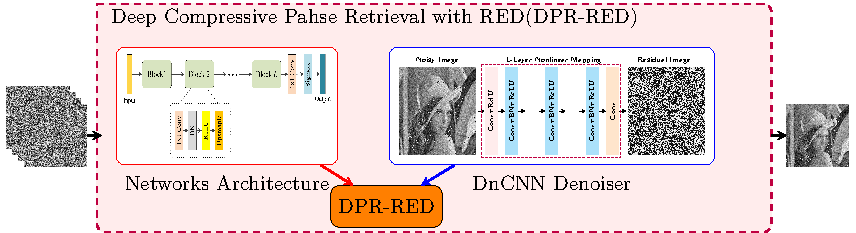
\includegraphics[width=\linewidth]{5-1}
	\caption{DPR-RED算法结构示意图}\label{fig:5-1}
\end{figure}

\section{深度图像先验}
随着深度神经网络的出现与发展,基于全监督学习的图像重建算法逐渐得到了广泛而深刻的应用,这些图像重建任务包括图像修复、去马赛克、去反光、去雾雪等\supercite{FanQingnan}。

虽然监督学习取得了巨大的成功,但其背后存在如下的问题:(1) 在图像去噪任务中,现有的全监督降噪网络,例如DnCNN、IRCNN、FFDNet、CBDNet等,它们往往需要在庞大的Noisy-Clean配对图像构成的数据集上训练,噪声图像人为的添加高斯噪声形成,其与真实图像的噪声存在较大的差异。因而在真实数据上的泛化性能往往十分糟糕;(2) 全监督学习取得高质量图像去噪性能取决于深度学习技术从海量的训练数据中学习到的先验知识具有更强的泛化能力和更复杂的参数化表达得到多数研究者的认可,这种观点仍存在不小的争议;(3) 全监督学习受限于训练集标签的数量与质量,在面对无标签、合成伪标签或者仅有弱标签的数据时,全监督学习的优势难以充分体现。

为了解决上述问题,研究者们提出了一系列具有开创性的工作。Ulyanovd等人另辟蹊径提出以未学习的深度神经网络U-Net作为图像先验引入图像去噪、单幅图像超分辨率、图像修复等基本问题,其性能已经超越人工创造的手工先验,如非局部相似性、稀疏性\supercite{Ulyanov,Mahendran,Tobias}等。不同于学习的深度生成先验,它不需要在海量数据集上进行任何训练,属于深度无监督学习的范畴。深度图像先验的核心思想在于生成器网络的结构足以在任何学习之前捕获图像的低频统计信息,从而实现类似HOG这样人为设计的特征提取。深度图像先验唯一的先验信息来自网络结构本身,而非通过神经网络学习获得的先验知识。深度图像先验的基本思想如下:

深度卷积神经网络可表示为含参的函数$x=T_{\Theta}(z)$,其中$z$表示来自编码分布空间的潜变量,例如生成对抗网络中的生成器从高斯分布采样以生成真实分布。一般线性图像反问题根据最大后验估计得到损失函数如下所示
\begin{equation} \label{problem:5-1}
	x^*=\arg\min_{x}E(x;y) + R(x).
\end{equation}
其中$E(x;y)=\frac{1}{2}\Vert{Hx-y}\Vert_2^2$表示退化模型的数据保真项,$R(x)$代表图像固有的先验知识。深度图像先验隐式地将$R(x)$嵌入到退化模型的数据保真项中,其数学表示如下
\begin{equation} \label{problem:5-2}
	\Theta^*=\arg\min_{\Theta}E(T_{\Theta}(z);y), 
\end{equation}
上述优化问题利用SGD或Adam优化器求得局部最优解$\Theta^*$,则重构图像由$x^*=T_{\Theta^*}(z)$生成。

\section{基于深度图像先验融合RED正则项的压缩相位恢复算法}
压缩感知的研究进展提供了线性测量最优采样复杂度下稀疏信号的重建算法,但这种方法对于非线性的反问题,已经遇到了潜在的基本采样复杂度瓶颈问题,即最优采样复杂度下界问题。在压缩相位恢复应用中,现有的基于稀疏表示的压缩相位恢复算法不能在最优非线性采样复杂度下重构原始信号。为了解决上述问题,学者们基于深度学习技术提出了不同的压缩相位恢复算法。最近的研究成果如下:

(1)Hand等人提出了基于深度生成先验的压缩相位恢复算法应用于欠采样的观测值\supercite{Hand}。给定预训练的生成器$G$,则压缩相位恢复问题相应的非凸优化问题为:
\begin{equation} \label{problem:5-3}
	z^*=\arg\min_{x}\frac{1}{2}\Vert{y-\vert{AG(z)}\vert}\Vert_2^2.
\end{equation}
上述优化问题的数值解严重依赖于潜变量$z$的初始化,并且在梯度下降迭代陷入局部最优无法逃离。式\eqref{problem:5-3}求得局部最优解之后,通过\eqref{equation:5-1}估计重构图像:
\begin{equation} \label{equation:5-1}
	\hat{x}=G(z^*).
\end{equation}

(2)Jagatap等人提出了基于深度图像先验DPG的压缩相位恢复算法:Net-GD与Net-PGD\supercite{Jagatap}。其相应的优化问题为:
\begin{equation} \label{problem:5-4}
	\min_{w}\quad \frac{1}{2}\Vert{y-\vert{Ax}\vert}\Vert_2^2\quad s.t.\quad x=G(w,z).
\end{equation}
该算法在较低采样率的情况下重构图像质量优于基于稀疏先验的压缩相位恢复算法(TVAL3、lasso)。在观测矩阵服从高斯分布并且满足RIP(Restricted Isometry Property)假设下,证明该算法收敛性与最优采样复杂度的下界。

本章受到Mataev等人DeepRED工作的启发\supercite{Mataev},本章提出了DPR-RED算法。该算法将RED先验作为正则项融入到深度图像先验损失函数中,其对应的优化问题为
\begin{equation} \label{problem:5-5}
	\begin{aligned} 
		\mathop{\text{minimize}}\limits_{x,\Theta}\quad&\frac{1}{2}\Vert{\vert{AT_{\Theta}(z)}\vert-y}\Vert_2^2+\frac{\lambda}{2}x^\top(x-D_{\sigma}(x)) \\
		\text{subject\ to}\quad &x=T_{\Theta}(z). \\
	\end{aligned}
\end{equation}
利用ADMM算法对问题\eqref{problem:5-5}进行求解,式\eqref{problem:5-5}对应的增广拉格朗日函数为:
\begin{equation} \label{equation:5-2}
	L_{\rho}(x,u,\Theta)=\frac{1}{2}\Vert{\vert{AT_{\Theta}(z)}\vert-y}\Vert_2^2+\frac{\lambda}{2}x^\top(x-D_{\sigma}(x))+\frac{\rho}{2}\Vert{x-T_{\Theta}(z)}\Vert_2^2-\rho{u^\top(x-T_{\Theta}(z))}.
\end{equation}
其中$u$为朗格朗日乘子向量,$\rho$为惩罚参数,对式\ref{equation:5-2}进行配方得到
\begin{equation} \label{equation:5-3}
	L_{\rho}(x,u,\Theta)=\frac{1}{2}\Vert{\vert{AT_{\Theta}(z)}\vert-y}\Vert_2^2+\frac{\lambda}{2}x^\top(x-D_{\sigma}(x))+\frac{\rho}{2}\Vert{x-T_{\Theta}(z)-u}\Vert_2^2.
\end{equation}
具体地,ADMM方法通过求解以下子问题(对于第$k+1$次迭代)对上述优化问题进行求解:

(1)更新网络参数$\Theta$:固定$x,u$,问题\eqref{equation:5-3}相当于求解以下子问题:
\begin{equation} \label{equation:5-4}
	\Theta^*=\arg\min_{\Theta}\frac{1}{2}\Vert{\vert{AT_{\Theta}(z)}\vert-y}\Vert_2^2+\frac{\rho}{2}\Vert{x-T_{\Theta}(z)-u}\Vert_2^2.
\end{equation}
式\eqref{equation:5-4}作为神经网络的损失函数,可用反向传播进行参数更新。

(2)重构图像$x$:固定$\Theta,u$,问题\eqref{equation:5-3}相当于求解以下子问题:
\begin{equation} \label{equation:5-5}
	x^*=\arg\min_{x}\frac{\lambda}{2}x^\top(x-D_{\sigma}(x))+\frac{\rho}{2}\Vert{x-T_{\Theta}(z)-u}\Vert_2^2.
\end{equation}
对式\eqref{equation:5-5}求梯度的得到:
\begin{equation} \label{equation:5-6}
	\lambda{(x-D_{\sigma}(x))}+\rho(x-T_{\Theta}(z)-u)=0.
\end{equation}
利用不动点迭代将式\eqref{equation:5-6}转化为
\begin{equation} \label{equation:5-7}
	\lambda{(x^{j+1}-D_{\sigma}(x^{j}))}+\rho(x^{j+1}-T_{\Theta}(z)-u)=0.
\end{equation}
所以第$k+1$次迭代为
\begin{equation} \label{equation:5-8}
	x^{j+1}:=\frac{1}{\lambda+\rho}(\lambda{D_{\sigma}(x^j)}+\rho(T_{\Theta}(z)+u)).
\end{equation}

(3)尺度对偶变量$u$更新:
\begin{equation} \label{equation:5-9}
	u^{k+1}:=u^k-x^{k+1}+T_{\Theta^{k+1}}(z).
\end{equation}

需要注意的是:(1)早停技术(early stopping):DPR-RED算法当重构图像的PSNR达到最大时,应停止迭代,避免过拟合的出现;(2)式\eqref{equation:5-4}的更新步数应比式\eqref{equation:5-8}快10次左右,以保证算法的稳健性。算法\ref{algorithm:5-1}总结了DPR-RED算法的实现细节。
\begin{algorithm}[!htbp]
	\setstretch{1.4}\zihao{-4}
	\caption{DPR-RED}
	\label{algorithm:5-1}
	\begin{algorithmic}[1]
		\REQUIRE	观测值$y\in \mathbb{R}^m$; % this command shows "Input"
		\ENSURE		% this command shows "Initialized"
		$\lambda,\rho>0, J=1, u^0=0, (x^0,\Theta^0)$随机; \\
		
		\WHILE {\emph{not converged}}
		\STATE	Update $\Theta^{k+1}$:Solve Equation \eqref{equation:5-4} using Adam; \\  % line number at left side
		\STATE	Update $x^{k+1}$:Through the fixed point \eqref{equation:5-8} for J iterations; \\	% line number at left side
		\STATE	Update $u^{k+1}$:$u^{k+1}:=u^k-x^{k+1}+T_{\Theta^{k+1}}(z)$; \\ % line number at left side
		\ENDWHILE
		\RETURN 重构图像$x^{k+1}$. % this command shows "Output"
	\end{algorithmic}
\end{algorithm}

在DPR-RED算法中,去噪器与网络参数更新并行如图\ref{fig:5-2}所示。
图\ref{fig:5-2}表明神经网络参数$\Theta$的更新可与去噪步骤并行执行,但Python的多线程对于CPU密集型任务无能为力,不能实现反向传播与去噪算子迭代的真正并行处理。
\begin{figure}[!hptb]
	\centering
	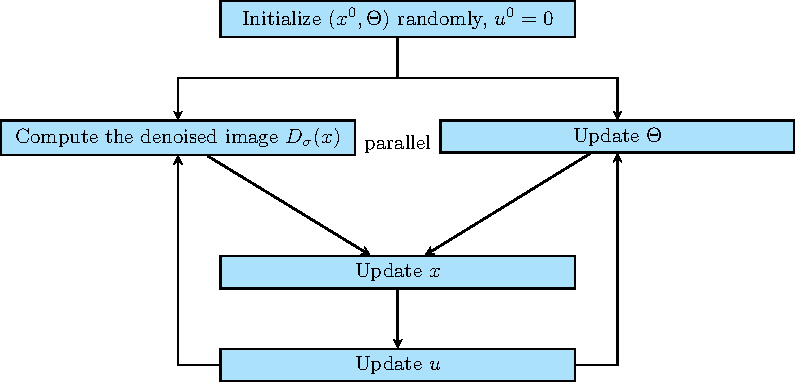
\includegraphics[width=0.8\linewidth]{5-2}
	\caption{去噪器与网络参数更新并行示意图}
	\label{fig:5-2}
\end{figure}

\section{实验结果及分析}
本章实验仿真设置如下:

(1)测试数据:测试图像来自于MNIST与CelebA数据集,包括归一化的6张28x28的灰度数字图像与5张64x64x3的RGB人脸图像;

(2)网络结构:对于MNIST,$x=T_{\Theta}(z)$采用编码-解码网络中的解码网络,$k_1=25,k_2=15,k_3=10$;对于CelebA采用$k_1=120,k_2=25,k_3=15,k_4=10$;

(3)DPR-RED算法参数设置:$\lambda=0.5,\rho=1,\sigma=3$,学习率为$1e-3$,迭代次数为$1e4$。为保证对比公平性,DPR算法的学习率与迭代次数与DPR-RED算法保持一致。

(4)观测矩阵:观测矩阵$A$的列向量为$\{a_j\overset{\underset{\mathrm{iid}}{}}{\sim}\mathcal{N}(0,I_n)\}_{1\leq{j\leq{m}}}$,采样率$m/n$取0.3,0.6,1;

(5)实验仿真平台:Intel(R) Xeon(R) CPU E5-2650 v4处理器(2.20GHz),252G内存,ubuntu 16.04操作系统, Tesla K80显卡,cuda 10.2,cudnn 7605。

\subsection{无噪声情况下的压缩相位恢复}
为了进一步验证DPR-RED算法的有效性,本节在不同欠采样率下对无噪声的观测值进行相位恢复,表\ref{table:5-1}与表\ref{table:5-2}为DPR算法与RED算法在MNIST/CelebA上的PSNR/SSIM比较结果。在MNIST数据集上,采样率为0.3,0.6,1.0时DPR-RED算法的PSNR分别比DPR高0.98db,0.48db,0.93db。上述对比表明DPR-RED算法的重构性能优于DPR算法,但不保证在其他的测试集上的反例出现。在CelebA数据集上,采样率为0.3,0.6,1.0时DPR-RED算法的PSNR分别比DPR高1.32db,0.45db,0.49db。上述对比表明DPR-RED算法的重构性能优于DPR算法,且在较低采样率下,DPR-RED算法更具优势。
\begin{table}[!htbp]
	\def\arraystretch{1.4}\centering\zihao{5}
	\caption{不同欠采样率下算法在MNIST上获得的平均PSNR(dB)/SSIM比较}
	\label{table:5-1}
	\begin{tabular*}{\linewidth}{@{}@{\extracolsep{\fill}}cccc@{}}
		\toprule
		采样率$m/n$   & 0.3 & 0.6 & 1.0\\ %\cmidrule(r){2-4}
		\midrule
		DPR           & 15.57/0.5131   & 25.32/0.9137  & 25.00/0.9129 \\
		DPR-RED       & {\color{red}16.55/0.5469}   & {\color{red}25.82/0.9228}  & {\color{red}25.93/0.9188} \\
		\bottomrule
	\end{tabular*}
\end{table}
\begin{table}[!htbp]
	\def\arraystretch{1.4}\centering\zihao{5}
	\caption{不同欠采样率下算法在CelebA上获得的平均PSNR(dB)/SSIM比较}
	\label{table:5-2}
	\begin{tabular*}{\linewidth}{@{}@{\extracolsep{\fill}}cccc@{}}
		\toprule
		采样率$m/n$    & 0.3 & 0.6 & 1.0 \\ %\cmidrule(r){2-4}
		\midrule
		DPR           & 27.71/0.8500   & 27.75/0.8539  & 28.18/0.8677 \\
		DPR-RED       & {\color{red}29.03/0.8616}   & {\color{red}28.20/0.8689}  & {\color{red}28.67/0.8766} \\
		\bottomrule
	\end{tabular*}
\end{table}
\begin{figure}[!htbp]
	\centering
	\subfigure[原始图像]{
		\begin{minipage}[t]{\linewidth}
			\centering
			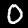
\includegraphics[width=0.08\linewidth]{mnist1}
			
\includegraphics[width=0.08\linewidth]{mnist2}
			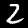
\includegraphics[width=0.08\linewidth]{mnist3}
			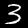
\includegraphics[width=0.08\linewidth]{mnist4}
			
\includegraphics[width=0.08\linewidth]{mnist5}
			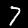
\includegraphics[width=0.08\linewidth]{mnist6}
			%\caption{fig}
		\end{minipage}
	}\vspace{-0.02\linewidth}
	\\
	\subfigure[DPR算法重构结果图]{
		\begin{minipage}[t]{\linewidth}
			\centering
			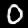
\includegraphics[width=0.08\linewidth]{5-3-1}
			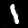
\includegraphics[width=0.08\linewidth]{5-3-2}
			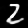
\includegraphics[width=0.08\linewidth]{5-3-3}
			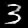
\includegraphics[width=0.08\linewidth]{5-3-4}
			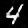
\includegraphics[width=0.08\linewidth]{5-3-5}
			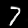
\includegraphics[width=0.08\linewidth]{5-3-6}
			%\caption{fig}
		\end{minipage}
	}\vspace{-0.02\linewidth}
	\\
	\subfigure[DPR-RED算法重构结果图]{
		\begin{minipage}[t]{\linewidth}
			\centering
			
\includegraphics[width=0.08\linewidth]{5-3-7}
			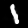
\includegraphics[width=0.08\linewidth]{5-3-8}
			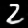
\includegraphics[width=0.08\linewidth]{5-3-9}
			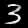
\includegraphics[width=0.08\linewidth]{5-3-10}
			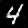
\includegraphics[width=0.08\linewidth]{5-3-11}
			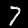
\includegraphics[width=0.08\linewidth]{5-3-12}
			%\caption{fig}
		\end{minipage}
	}
	\caption{DPR与DPR-RED在MNIST上采样率为$m/n=0.6$时的重构结果} 
	\label{fig:5-3} 
\end{figure}
\begin{figure}[!htbp]
	\vspace{-0.03\linewidth}
	\centering
	\subfigure[原始图像]{
		\begin{minipage}[t]{\linewidth}
			\centering
			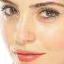
\includegraphics[width=0.1\linewidth]{celeba1}
			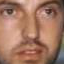
\includegraphics[width=0.1\linewidth]{celeba2}
			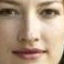
\includegraphics[width=0.1\linewidth]{celeba3}
			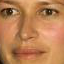
\includegraphics[width=0.1\linewidth]{celeba4}
			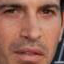
\includegraphics[width=0.1\linewidth]{celeba5}
			%\caption{fig}
		\end{minipage}
	}\vspace{-0.02\linewidth}
	\\
	\subfigure[DPR算法重构结果]{
		\begin{minipage}[t]{\linewidth}
			\centering
			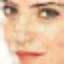
\includegraphics[width=0.1\linewidth]{5-4-1}
			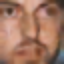
\includegraphics[width=0.1\linewidth]{5-4-2}
			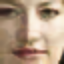
\includegraphics[width=0.1\linewidth]{5-4-3}
			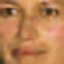
\includegraphics[width=0.1\linewidth]{5-4-4}
			
\includegraphics[width=0.1\linewidth]{5-4-5}
			%\caption{fig}
		\end{minipage}
	}\vspace{-0.02\linewidth}
	\\
	\subfigure[DPR-RED算法重构结果]{
		\begin{minipage}[t]{\linewidth}
			\centering
			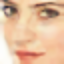
\includegraphics[width=0.1\linewidth]{5-4-6}
			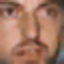
\includegraphics[width=0.1\linewidth]{5-4-7}
			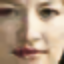
\includegraphics[width=0.1\linewidth]{5-4-8}
			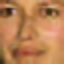
\includegraphics[width=0.1\linewidth]{5-4-9}
			
\includegraphics[width=0.1\linewidth]{5-4-10}
			%\caption{fig}
		\end{minipage}
	}
	\caption{DPR与DPR-RED在CelebA上采样率为$m/n=0.3$时的重构结果} 
	\label{fig:5-4}  
\end{figure}

为了从主观视觉上比较了不同算法的性能,图\ref{fig:5-3}与图\ref{fig:5-4}给出了测试图像的重构结果。图\ref{fig:5-3}显示了在采样率为0.6时MNIST手写体数字图像的重构结果,图\ref{fig:5-4}是采样率为0.3时CelebA人脸图像的重构结果。图\ref{fig:5-3}因手写体图像模式过于简单,无法从主观视觉上区分两种算法的优劣。但是对于图\ref{fig:5-4},可以看出DPR-RED算法在低采样率重构出了比DPR算法更加清晰的人脸轮廓与细节。

\subsection{含噪情况下的压缩相位恢复}
本节设置高斯噪声SNR=15dB,泊松噪声强度$\alpha=81$。图\ref{fig:5-5}与图\ref{fig:5-6}分别给出了DPR算法与DPR-RED算法在MNIST与CelebA测试集上的重构结果。
\begin{figure}[!htbp]	
	\centering
	\subfigure[原始图像]{
		\begin{minipage}[t]{\linewidth}
			\centering
			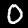
\includegraphics[width=0.1\linewidth]{mnist1}
			
\includegraphics[width=0.1\linewidth]{mnist2}
			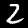
\includegraphics[width=0.1\linewidth]{mnist3}
			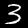
\includegraphics[width=0.1\linewidth]{mnist4}
			
\includegraphics[width=0.1\linewidth]{mnist5}
			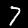
\includegraphics[width=0.1\linewidth]{mnist6}
			%\caption{fig}
		\end{minipage}
	}
	\\
	\subfigure[DPR算法重构结果]{
		\begin{minipage}[t]{\linewidth}
			\centering
			
\includegraphics[width=0.1\linewidth]{5-6-1}
			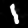
\includegraphics[width=0.1\linewidth]{5-6-2}
			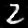
\includegraphics[width=0.1\linewidth]{5-6-3}
			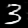
\includegraphics[width=0.1\linewidth]{5-6-4}
			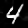
\includegraphics[width=0.1\linewidth]{5-6-5}
			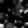
\includegraphics[width=0.1\linewidth]{5-6-6}
			%\caption{fig}
		\end{minipage}
	}
	\\
	\subfigure[DPR-RED算法重构结果]{
		\begin{minipage}[t]{\linewidth}
			\centering
			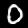
\includegraphics[width=0.1\linewidth]{5-6-7}
			
\includegraphics[width=0.1\linewidth]{5-6-8}
			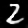
\includegraphics[width=0.1\linewidth]{5-6-9}
			\includegraphics[width=0.1\linewidth]{5-6-10}
			\includegraphics[width=0.1\linewidth]{5-6-11}
			\includegraphics[width=0.1\linewidth]{5-6-12}
			%\caption{fig}
		\end{minipage}
	}
	\caption{DPR与DPR-RED在SNR=15dB采样率为$m/n=0.6$时的重构结果} 
	\label{fig:5-5} 
\end{figure}
\begin{figure}[!hptb]		
	\centering
	\subfigure[原始图像]{
		\begin{minipage}[t]{\linewidth}
			\centering
			\includegraphics[width=0.1\linewidth]{mnist1}
			\includegraphics[width=0.1\linewidth]{mnist2}
			\includegraphics[width=0.1\linewidth]{mnist3}
			\includegraphics[width=0.1\linewidth]{mnist4}
			\includegraphics[width=0.1\linewidth]{mnist5}
			\includegraphics[width=0.1\linewidth]{mnist6}
			%\caption{fig}
		\end{minipage}
	}
	\\
	\subfigure[DPR算法重构结果]{
		\begin{minipage}[t]{\linewidth}
			\centering
			\includegraphics[width=0.1\linewidth]{5-7-1}
			\includegraphics[width=0.1\linewidth]{5-7-2}
			\includegraphics[width=0.1\linewidth]{5-7-3}
			\includegraphics[width=0.1\linewidth]{5-7-4}
			\includegraphics[width=0.1\linewidth]{5-7-5}
			\includegraphics[width=0.1\linewidth]{5-7-6}
			%\caption{fig}
		\end{minipage}
	}
	\\
	\subfigure[DPR-RED算法重构结果]{
		\begin{minipage}[t]{\linewidth}
			\centering
			\includegraphics[width=0.1\linewidth]{5-7-7}
			\includegraphics[width=0.1\linewidth]{5-7-8}
			\includegraphics[width=0.1\linewidth]{5-7-9}
			\includegraphics[width=0.1\linewidth]{5-7-10}
			\includegraphics[width=0.1\linewidth]{5-7-11}
			\includegraphics[width=0.1\linewidth]{5-7-12}
			%\caption{fig}
		\end{minipage}
	}
	\caption{DPR与DPR-RED在$alpha=81$采样率为$m/n=0.6$时的重构结果}
	\label{fig:5-6} 
\end{figure}

在观测值高斯噪声占比SNR=15dB与泊松噪声强度$\alpha=81$均为观测值严重受到噪声污染的情况,从图\ref{fig:5-5}与\ref{fig:5-6}可以看出,手写体数字``7"在0.6的欠采样率下未被成功重构,这表明DPR-RED算法在噪声强度较大的情况下存在局限性,后期仍有巨大的改进空间。

\section{本章小结}
本章首先简述了深度图像先验的基本原理,然后提出了基于深度图像先验融合RED正则项的压缩相位恢复算法。该算法将显式的RED先验作为正则项添加到隐式的深度图像先验损失函数中,采用ADMM算法进行求解。实验证明该算法在欠采样率观测值下对含高斯与泊松噪声的观测值具有鲁棒性。

